\documentclass[type=bachelor]{thuthesis}
% 选项:
%   type=[bachelor|master|doctor|postdoctor], % 必选
%   secret,                                   % 可选
%   pifootnote,                               % 可选(建议打开)
%   openany|openright,                        % 可选,基本不用
%   arial,                                    % 可选,基本不用
%   arialtoc,                                 % 可选,基本不用
%   arialtitle                                % 可选,基本不用

% 所有其它可能用到的包都统一放到这里了,可以根据自己的实际添加或者删除。
\usepackage{thuthesis}
\usepackage{bm}
\newcommand{\transpose}[1]{\ensuremath{#1^{\scriptscriptstyle T}}}
\DeclareMathOperator*{\rgmax}{argmax}
\DeclareMathOperator*{\rgmin}{argmin}
\DeclareMathOperator{\Tr}{Tr}
% 定义所有的图片文件在 figures 子目录下
\graphicspath{{figures/}}

% 可以在这里修改配置文件中的定义。导言区可以使用中文。
\usepackage{listings}
\definecolor{dkgreen}{rgb}{0,0.6,0}
\definecolor{gray}{rgb}{0.5,0.5,0.5}
\definecolor{mauve}{rgb}{0.58,0,0.82}
\lstset{
  frame=tb,
  aboveskip=3mm,
  belowskip=3mm,
  showstringspaces=false,
  columns=flexible,
  framerule=1pt,
  rulecolor=\color{gray!35},
  backgroundcolor=\color{gray!5},
  basicstyle={\small\ttfamily},
  numbers=none,
  numberstyle=\tiny\color{gray},
  keywordstyle=\color{blue},
  commentstyle=\color{dkgreen},
  stringstyle=\color{mauve},
  breaklines=true,
  breakatwhitespace=true,
  tabsize=3,
  title=\lstname
}
\begin{document}

%%% 封面部分
\frontmatter
\includepdf[pages=-]{data/CompetetionCover.pdf}
%\input{data/CompetitionCover}
% 如果使用授权说明扫描页,将可选参数中指定为扫描得到的 PDF 文件名,例如:
%\makecover

%% 目录
\tableofcontents

%% 符号对照表
\begin{denotation}[3cm]
\item[$h_a$] 无人机飞行高度
\item[$h_g$] 地面高度
\item[$\phi_e$] 无人机最大仰角
\item[$r_i$] 重点区域半径
\item[$r_t$] 无人机转弯半径
\item[$v_a$] 无人机平均飞行速度
\item[$r_{at}$] 无人机与通信终端之间的最大通信距离
\item[$r_{aa}$] 无人机与无人机之间的最大通信距离



\end{denotation}



%%% 正文部分
\mainmatter
\chapter{问题回顾}
\label{cha:question}

\section{问题重述}
%content
%research current state here
2017年8月8日,四川阿坝州九寨沟县发生7.0级地震,造成了不可挽回的人员伤亡和重大的财产损失。由于预测地震比较困难,及时高效的灾后救援是减少地震损失的重要措施。无人机作为一种新型运载工具,能够在救援行动中发挥重要作用。为提高其使用效率,请你们解决无人机优化运用的几个问题。
附件1给出了震区的高程数据,共有2913列,2775行。第一行第一列表示(0,0)点处的海拔高度值(单位:米),相邻单元格之间的距离为38.2米,即第m行第n列单元格中的数据代表坐标(38.2(m-1), 38.2(n-1))处的高度值。震区7个重点区域的中心位置如下表所示(单位:千米):
\begin{table}
\centering
\begin{tabular}{|c|c|c|}
\hline
中心点&X坐标&Y坐标\\
\hline
A&30.3&89.8\\
\hline
B&66.0&84.7\\
\hline
C&98.4&76.7\\
\hline
D&73.7&61.0\\
\hline
E&57.9&47.6\\
\hline
F&86.8&22.0\\
\hline
G&93.6&48.8\\
\hline
\end{tabular}
\end{table}
除另有说明外,本题中的无人机都假设平均飞行速度60千米/小时,最大续航时间为8小时,飞行时的转弯半径不小于100米,最大爬升(俯冲)角度为±15°,与其它障碍物(含地面)的安全飞行距离不小于50米,最大飞行高度为海拔5000米。所有无人机均按规划好的航路自主飞行,无须人工控制,完成任务后自动返回原基地。
\subsection{问题一:灾情巡查}
大地震发生后,及时了解灾区情况是制订救援方案的重要前提。为此,使用无人机携带视频采集装置巡查7个重点区域中心方圆10公里(并集记为S)以内的灾情。假设无人机飞行高度恒为4200米,将在地面某点看无人机的仰角大于60°且视线不被山体阻隔视为该点被巡查。若所有无人机均从基地H(110,0)(单位:千米)处派出,且完成任务后再回到H,希望在4小时之内使区域S内海拔3000米以下的地方尽可能多地被巡查到,最少需要多少架无人机?覆盖率是多少?每架无人机的飞行路线应如何设计?在论文中画出相应的飞行路线图及巡查到的区域(不同的无人机的飞行路线图用不同的颜色表示)。

进一步,为及时发现次生灾害,使用无人机在附件1给出的高度低于4000米的区域(不限于S)上空巡逻。问最少需要多少架无人机、如何设定每架无人机的飞行时间、路线,才能保证在72小时内,上述被巡查到的地方相邻两次被巡查的时间间隔不大于3小时(无人机均需从H出发并在8小时内回到H,再出发的时间间隔不小于1小时)?
\begin{figure}[!ht]
\centering
\includegraphics[width=6cm]{problem_1.png}
\end{figure}
\subsection{问题二:生命迹象探测}
使用无人机携带生命探测仪搜索生命迹象,能够给灾后救援提供准确的目标定位。拟从基地H(110,0),J(110,55)(单位:千米)处总共派出30架无人机(各15架),任务完成后回到各自的出发地。探测仪的有效探测距离不超过1000米,且最大侧视角(探测仪到可探测处的连线与铅垂线之间的夹角)为60度。请你们规划它们的飞行路线,使附件1所给出的全区域内海拔3000米以下部分能被探测到的面积尽可能大,且使从第一架无人机飞出到最后一架完成任务的无人机回到基地的时间间隔尽量短。
\begin{figure}[!ht]
\centering
\includegraphics[width=6cm]{problem_2.png}
\end{figure}
\subsection{问题三:灾区通信中继}
大地震发生后,地面电力设施被破坏,灾区通信中断。太阳能无人机(白天不受续航能力限制,其余条件同前述)
可以作为地面移动终端之间的通信中继,为灾区提供持续的通信保障(地面终端只能与无人机进行通信,
无人机之间只要不超过最大通信距离就可以互相通信,地面与地面之间的通信由无人机转接)。
假设无人机在空中飞行时,可与距离3000米以内的移动终端通信,无人机之间的最大通信距离为6000米,
问最少需要多少架无人机、每架无人机的飞行路线如何,才能保证在白天12小时内,
附件2中的任意两个地面终端之间都能实现不间断通信(作为中继的无人机之间的切换时间忽略不计,地面终端的移动距离不超过2千米)?
\subsection{问题四:无人机对地的数据传输}
指挥中心拟从H派出3架无人机携带通信装备向灾区内的72个地面终端(分布见附件2)发送内容不同,
总量均为500M(1M按$10^6$比特计算)的数据。设每台通信装备的总功率是5瓦,可同时向不超过10个地面终端发送数据。
数据传输过程可以简化为:当地面终端i看无人机的仰角大于30$^{\circ}$、距离不超过3000米且没有山体阻隔时,
如果无人机当前服务用户少于10个,则开始向i发送数据,并瞬间完成所有用户的功率再分配,
否则,搁置i的需求,直到有地面用户退出,若此时i仍在可服务区域,则为i服务(先到先服务)。
如果在一个服务时间区间(即无人机和终端之间满足可传输数据条件的时间范围)内不能传完全部数据,
则以后区间可以续传。再设i用户在时刻t接收到无人机发送的信息速率为
$r_i(t)=B_i \log\left(1+\frac{p_i(t)}{\rho_0 d^2(u,i)}\right)$(比特/秒),其中
$B_i$表示无人机服务 的子信道带宽(取值见附件2,单位Hz), 
$p_i(t)$表示t时刻无人机为第i个地面用户所在的子信道分配的功率,单位:w(瓦),
$d(u,i)$表示t时刻无人机与i之间的欧氏距离,单位:米。$\rho_0$为信道特性参数,为简单起见,
取为$4.314\times 10^{-10}$(单位略),假设无人机飞行速度在60~100千米/小时之间可调(水平面内最大加速度 $\pm 5m/s^2$,
铅垂面内最大加速$\pm 2m/s^2$,可同时在两个方向上加速),
请你们为无人机设计恰当的航线、速度以及所服务的用户,并为每一个用户分配恰当的功率,使得无人机完成所有任务的时间总和尽量短。
%focus
\section{文章结构}
本文在第 \ref{cha:model} 章中给出了问题1关于区域划分和无人机路径规划的数学模型。
本文在第 \ref{cha:com_model} 章中给出了问题3关于无人机作为通信中继的数学模型。
本文在第 \ref{appendix} 章中给出了我们求解问题1和3所使用的matlab代码。

\chapter{数学模型}
\label{cha:model}
根据地形数据作出该区域的等高线地形图如 所示
\begin{figure}[!ht]
\centering
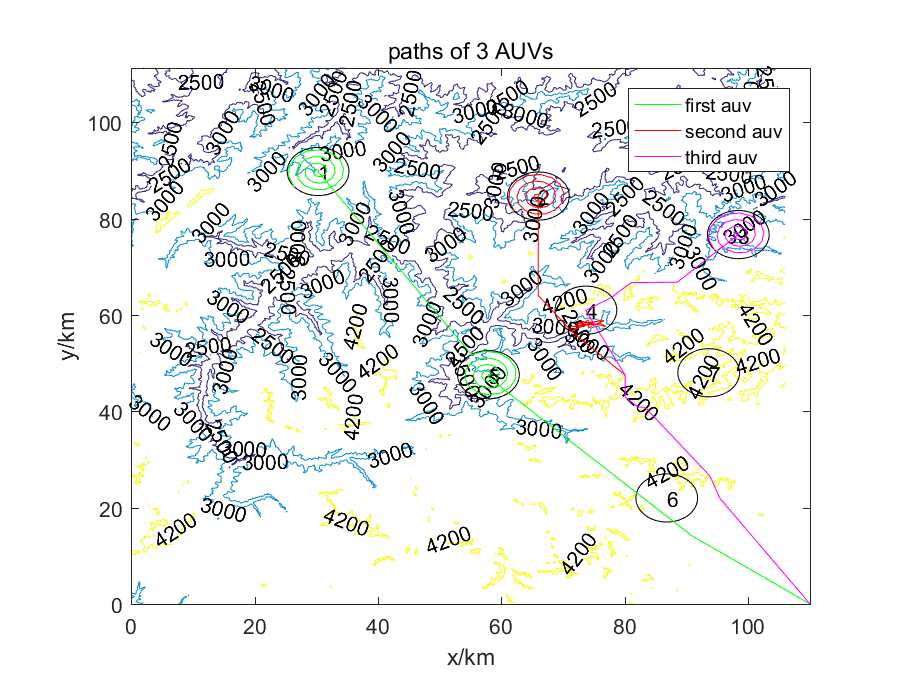
\includegraphics[width=18cm]{3path3.eps}
\caption{等高线地形图}\label{fig:3path}
\end{figure}

\section{模型假设}
\subsection{无人机路径规划算法选择}
对于单架无人机,希望其从指定起点到指点目标点的飞行时间最短。为此,我们将震区转化为二维网格,将高度超过4200米的地形区视为
障碍,在每一个网格的内部节点中,有8个相邻的节点,对于网格中的对角线的边,权值赋为$\sqrt{2}$,其余边为权值为1。
为此,我们给出如下的无人机路径规划方案:
\begin{enumerate}
\item 由震区地形数据建立图模型
\item 由图模型计算离散域的最短路径
\item 根据Visibility Graph 对离散域求出的最短路径进行优化并考虑到无人机飞行必须满足的约束条件对路径进行平滑
\end{enumerate}
\subsection{最大覆盖区域的优化算法选择}
最大覆盖区域的问题是NP难的问题,对于有高于4200米地形的重点区域,我们采用贪心算法对重点区域进行覆盖,该方法可在多项式时间内实现,
而且已有文献说明贪心法的平均覆盖率可达0.63\cite{Feige1998A}。贪心算法每次选取最低点并记录下已经巡逻到的区域,然后在未巡逻到3000米以下的区域
继续找最低点,直到巡逻区域在重点区域的比重达到设定的阀值。

在上述贪心方法找到若干个离散点后,若无人机遍历离散点,即可达到巡逻区域比例不低于上述阀值的效果。
为此,采用中国旅行商问题的思路规划出最短路径,求解中国旅行商问题采用整数规划的方法,并用增加不等式约束多次迭代
的方法消除子回路。由于离散点数目较少,完全图的规模较小,故该求解方法可行。
对于重点区域4使用上述方法求出20个圆的覆盖率达到$96\%$以上。并用整数规划的方法求出遍历这20个圆的圆心的
最短路径如图 \ref{fig:region4}所示
\begin{figure}[!ht]
\centering
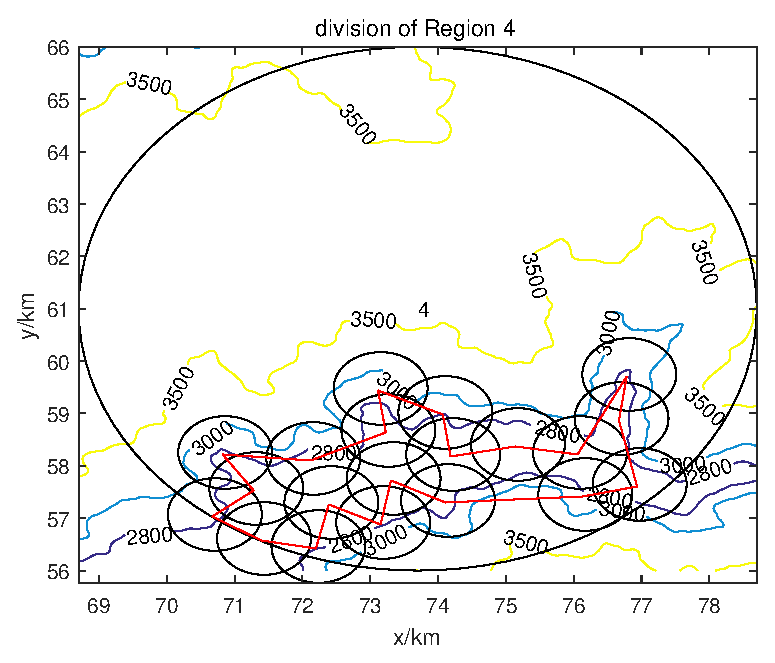
\includegraphics[width=10cm]{region4.eps}
\caption{重点区域4三千米以下位置的遍历路径}\label{fig:region4}
\end{figure}

对于全部低于4200米地形的重点区域,可以实现全覆盖。为此我们先让无人机飞到目标区域的圆心,
并采用阿基米德螺旋线的方式进行巡查。由于阿基米德螺旋线具有从起点出发的射线与螺旋线交点等距的性质,相比其它飞行轨迹
实现全覆盖用时较短。
以螺旋线起点为极坐标原点,则旋线方程为:
\begin{equation}
r=b\theta
\end{equation}
分隔距离为
\begin{equation}
d=2\pi b
\end{equation}
对于低于4200米地形区域(A,B,C,E)之一,记其最大高度为$h_g$,无人机飞行高度记为$h_a$, 则覆盖半径的最小值为
\begin{equation}
r_{\text{min}}=\tan(\phi_e/2)(h_a-h_g)
\end{equation}
取 $d=2r_{\text{min}}$ 可保证无人机按螺旋线飞行可实现自圆心向外区域的全部覆盖。无人机飞行所需的最小角度为
\begin{equation}\label{eq:thetaMin}
\theta_{\text{min}}=\frac{r_i-r_{\text{min}}}{b}
\end{equation}

%为保证螺旋线转过第一个$360^{\circ}$时可以覆盖图(\ref{fig:SpiralCenter})所示的区域,要求
%\begin{figure}[!ht]\label{fig:SpiralCenter}
%\centering
%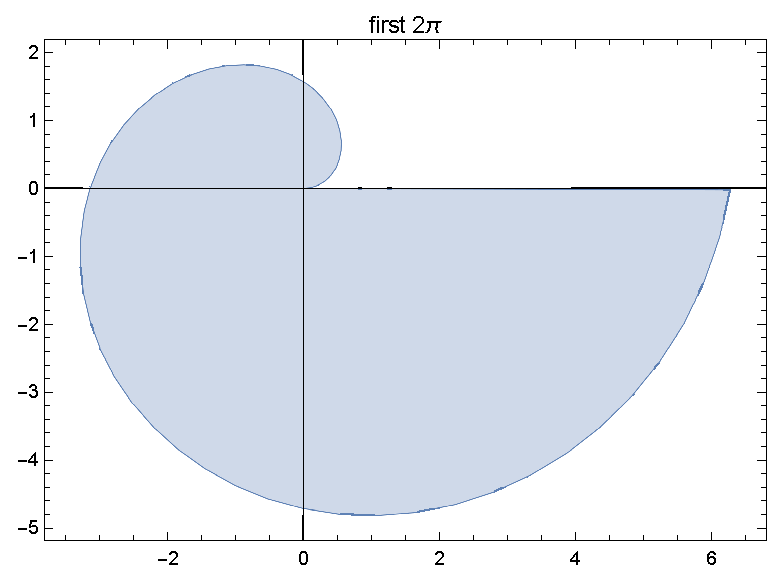
\includegraphics[width=6cm]{spiralCenter.eps}
%\caption{$r\leq b,\theta\leq 2\pi$}
%\end{figure}
为保证无人机转弯半径的要求,即螺旋线上任一点的曲率半径$\rho$大于$r_t$,即
\begin{equation}
\frac{b(\theta^2+1)^{\frac{3}{2}}}{\theta^2+2}\geq r_t
\end{equation}
对于螺旋线,我们取$\theta$从$\pi$开始,上式约束即为:
\begin{equation}
\frac{b(\pi^2+1)^{\frac{3}{2}}}{\pi^2+2}\geq r_t
\end{equation}
而对于$[0,\pi]$之间的飞行曲线,由于距离较短,无人机可调整方向进入螺旋线轨道。用时按$\frac{b\pi}{v_a}$近似。
根据螺旋线的弧长公式
\begin{equation}
s(\theta)=\frac{1}{2}b(\theta\sqrt{1+\theta^2}+\sinh^{-1}\theta)
\end{equation}
代入\eqref{eq:thetaMin}中的最小角度即可求出最小飞行距离$s_{\text{min}}$,除以无人机的速度$v_a$即可得飞行时间。
%关于极轴方向选取的任意性。
\section{实际计算中的近似}
%计算覆盖区域时做的近似:
\begin{itemize}
\item 无人机飞行折线的近似
\item 路径规划问题转化为图模型时只考虑无人机沿坐标轴与对角线方向的飞行
\item 只按最大俯角计算覆盖区域时忽略了能见范围内可能存在的地形遮挡
\end{itemize}
\subsection{平滑算法}
对于无人机飞行折线的近似,在所有折线的拐角处,我们按拐角的大小分如下两种情况对飞行曲线进行平滑以满足最小飞行半径的要求:
$\theta<80^{\circ}$,这时飞机曲线转弯用时比折线用时更长,多出的时间为
\begin{equation}
\Delta t=r_t(\pi+\theta-\tan\theta)
\end{equation}
示意图如下:
\begin{figure}[!ht]\label{fig:smaller}
\centering
\includegraphics[width=6cm]{smaller.jpg}
\caption{$\theta<80^{\circ}$}
\end{figure}

$\theta>80^{\circ}$,用外接圆弧对折线进行平滑,这时飞机曲线转弯用时比折线用时更短$\Delta t<0$,
\begin{equation}
\Delta t=r_t(\frac{2}{\tan (\theta/2)}-\pi+\theta)
\end{equation}
示意图如下:
\begin{figure}[!ht]\label{fig:larger}
\centering
\includegraphics[width=6cm]{larger.jpg}
\caption{$\theta>80^{\circ}$}
\end{figure}

\subsection{Theta Star 算法}
我们在路径规划中,使用dijkstra 算法求图中两点的最短路径。理论上原问题中任意可直达的两点均需转化为一条边,且需要全局考虑。
但这样做计算开销过大,因此我们采用只考虑正方形边和对角线的方式,这样求出的图中的最短路径并非是原问题的最短路径,因为这时的路径的
方向角只能取 $0,45^{\circ},90^{\circ},135^{\circ}$ 这几个有限的值。我们针对求出的路径进行后处理,通过对路径的折线拐点根据是否可直达
重建一个小规模的图再次使用dijkstra 算法求最短路径,从而大幅减少了最终折线拐点的数量。

关于判断地图中两点是否可直达的算法,我们借用计算机图形学在栅格点画直线的方法\cite{Bresenham1965Algorithm},可避免浮点数运算,时间复杂度是$O(n)$。

针对图中的最短路径并非是原问题的最短路径这一问题,文献\cite{Nash2014Theta} 给出了一种在规划最短路径时不局限于图的边的方法,以取代A star等方法需要
后处理的随意性,在我们的模型中,我们也考虑使用 Theta Star 算法,由于整个算法用matlab 纯脚本实现,难以使用优先队列等数据结构对算法进行优化,
因此对于规模较大的问题运算过慢,这里只作为一种替代方法提出。

\subsection{地形遮挡}
给定无人机的空间位置求解其覆盖区域时,我们采用的是比较无人机附近的点的圆锥投影侧面上的点是否在地形之上的方法。这样做避免了空间上判断
视距的问题,使单次判别的复杂度由$O(n)$降到$O(1)$,但有可能忽略了中间的地形遮挡而存在误判,考虑到地形起伏的连续性及问题的实际参数,误判相对较小,因此我们采用
锥面投影的方法作为求覆盖区域的主要方法。

根据上面的说明,我们计算出重点区域4,6内没有3000米以下的地方,因此无人机无需飞往。
对于其他5个重点区域,至少需要3架无人机可使全部重点区域的3000米以下的地方覆盖率达到$100\%$,
其飞行路线如图 \ref{fig:3path} 所示,其中第一架无人机负责巡逻区域5和区域1,
用时3.82小时;第二架无人机负责巡逻区域4和区域2,用时3.14小时;第三架
无人机负责巡逻区域3,用时2.66小时。

\section{区域全部覆盖时的补充}
\subsection{稀疏采样}
求解全部覆盖区域时由于格点过密,难以全局直接用图论的方法求解。我们首先根据无人机的覆盖区域对整个区域进行重采样,得到原格点数$\frac{1}{25}$的样本点,
若多架无人机全部遍历这些点,则可实现对整个区域的覆盖。

针对全部求出的点,可以采用 VRP (Vehicle Routing Problem) 的方法对给定的无人机数量进行路径规划。由于时间和能力所限,
我们在这方面仅仅做了一些文献调研并提出一些初步的设想:

对于大规模的VRP问题,难以精确求解,需要采用近似算法,如遗传算法或模拟退火\cite{Kirkpatrick1983Optimization}的方法,
其中模拟退火的方法从一组可行解出发,通过随机选取这组可行解的邻居解,通过比较两组解对应的代价函数的大小按一定概率
决定是否进行状态转移,由于本问可行解不易构造,由于地形的限制,邻居解难以刻画,故我们暂时没有想到如何求解该问题。


\chapter{通信中继的数学模型}
\label{cha:com_model}
由于地面终端只能与无人机通信,故在等效图模型中其度为1,先假设地面终端静止,如果存在一种无人机的部署方案使得整部图连通,那么
根据最小生成树的理论,通过去掉一些边仍能保证整部图连通,所以我们只需考虑构造一个树结构使得所有地面终端作为树的叶节点。

采用归纳的方法构造树,先假设对给定的$n$个地面终端已经存在$m$架无人机满足条件。考虑新增一个地面终端$t_j$,
那么我们先考虑离新增的地面终端最近的无人机$a_i$,在不破坏原有树的连通性的前提下移动$a_i$更靠近$t_j$,
如果$a_i$的移动可以满足在与$t_j$通信的范围内,则本轮结束;如果移动完$a_i$仍不能满足要求,顺次考虑其他所有无人机;
如果所有无人机都不能满足要求,保留移动后离$t_j$最近的那架无人机$a_k$的移动方案
并在$a_k$与$t_j$的连线上增加相应数量的
无人机使得条件成立。如此继续下去,可给出全部$N$个地面终端所需的无人机的静态部署方案。

这里问题的难点在于如何刻画“不破坏原有树的连通性”,特别是求出$a_i$可移动的范围。分两种情况考虑:
如果存在某个地面终端通信半径内只有$a_i$,那么$a_i$不能脱离该通信半径$r_{at}$划定的圆;否则则不受此约束。
对于$a_i$所连的任意两架无人机之间的距离如果超过$r_{aa}$,那么该无人机不能脱离两架无人机最大通信圆的相交区域。
可以通过不等式描述这些区域,因此子问题变成如下的平面上的几何优化问题:
\begin{proposition}
设目标点$\bm{P}=(x_0,y_0)$,某地面终端坐标为$(x_1,y_1)$,某其他两架无人机坐标为$(x_2,y_2),(x_3,y_3)$
求解
\begin{equation}\label{bilevel}
\left\{\begin{array}{l}
\min\limits_{{\mbox{\footnotesize\boldmath $x$}}} \sqrt{(x-x_0)^2+(y-y_0)^2}\\[0.2cm]
\mbox{subject to:}\\[0.1cm]
\qquad \left\{\begin{array}{l}
        \sqrt{(x-x_1)^2+(y-y_1)^2}\le r_{at}\\[0.1cm]
        \dots \\[0.1cm]
      \end{array}\right.
\qquad \left\{
    \begin{array}{l}
    \sqrt{(x-x_2)^2+(y-y_2)^2}\le r_{aa}\\[0.2cm]    
    \sqrt{(x-x_3)^2+(y-y_3)^2}\le r_{aa}\\[0.2cm]
    \dots
    \end{array}\right.
\end{array}\right.
\end{equation}
\end{proposition}

实际计算中,由于该子优化问题需要在循环内部调用,实现起来比较复杂,由于时间所限,我们没有完全实现上面描述的算法,而采用的是
当新增加的地面终端的位置不在现有的无人机覆盖范围之内时,在离该地面终端最近的无人机与该地面终端之间增加相应数量的无人机以满足
通信要求。当我们的场景变为动态场景时,只需将无人机与地面终端的通信距离$r_{at}$等效为 1km 即可。

根据简化后的方法求出的无人机的部署方案如下图所示:
\begin{figure}[!ht]\label{fig:communicaton}
\centering
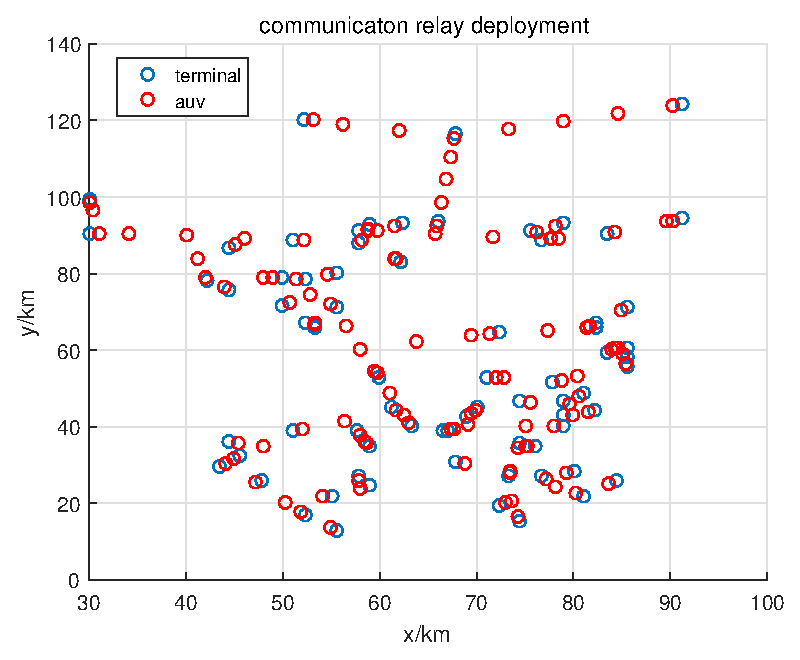
\includegraphics[width=10cm]{communicaton_relay_deployment.eps}
\caption{无人机的部署方案}
\end{figure}

所需的无人机数量是115架,这是一个上界。

%\include{data/myChap04Content}
%\include{data/myChap05Content}%conclusion
%%% 其它部分
%\backmatter

%% 本科生要这几个索引,研究生不要。选择性留下。
% 插图索引
\listoffigures
%\listofequations


%% 参考文献
% 注意:至少需要引用一篇参考文献,否则下面两行可能引起编译错误。
% 如果不需要参考文献,请将下面两行删除或注释掉。


%% 致谢
%\include{data/myAck}

%% 附录
\chapter{附录}\label{appendix}
\section{求解使用的代码}
\lstinputlisting[language=]{../launcher.m}
\lstinputlisting[language=]{../LineOfSight.m}
\lstinputlisting[language=]{../shortest_path.m}
\lstinputlisting[language=]{../user_plot_global.m}
\lstinputlisting[language=]{../user_plot_local.m}
\lstinputlisting[language=]{../region_traverse.m}
\lstinputlisting[language=]{../min_pos.m}
\lstinputlisting[language=]{../compute_time.m}
\lstinputlisting[language=]{../index_to_pos.m}
\lstinputlisting[language=]{../pos_to_index.m}
\lstinputlisting[language=]{../theta_star.m}
\lstinputlisting[language=]{../communication.m}
\lstinputlisting[language=]{../circle_constraint.m}
%\input{data/myAppendix}

\bibliographystyle{thuthesis}
\bibliography{ref/refs}

%% 本科生进行格式审查是需要下面这个表格,答辩可能不需要。选择性留下。
% 综合论文训练记录表
%\includepdf[pages=-]{scan-record.pdf}
\end{document}
